\documentclass{article}
\usepackage{graphicx}
\usepackage{float}

\title{Documentação do PI}
\author{Kauê José Abdalla Leal}
\date{30/05/2024}

\begin{document}

\maketitle

\begin{center}
      Izabela Tayná Reis Coimbra (PO)\\
      Kauê José Abdalla Leal (Design e Documentação)\\
      Isabela Maria de Oliveira (Back-End)\\
      Pedro Victor Virgino da Cunha (Front-End)\\
      Victor Ferreira Neves (Front-End e Back-End)
\end{center}

\newpage

\begin{center}
      \textbf{Documentação}
\end{center}


\section{Briefing}

Viajar, para muitos, é uma experiência transcendental, um momento de descoberta e aventura. No entanto, por trás da maravilha das paisagens exóticas e dos sorrisos em fotos, existe uma jornada de planejamento muitas vezes árdua e complexa. É nesse cenário desafiador que nasce nosso projeto: uma plataforma inovadora voltada para o planejamento de viagens, compartilhamento de experiências e dicas de economia.
Nossa história é moldada por diversos atores, cada um com seu papel único. Temos os viajantes individuais, sedentos por aventura e novas descobertas. Os grupos de viajantes, unidos pelo espírito de camaradagem e pela busca de experiências compartilhadas. E, é claro, nossa comunidade online de viajantes, o coração pulsante dessa jornada coletiva. O dilema é universal: escolher destinos, estimar custos, montar itinerários e enfrentar a barreira linguística são apenas alguns dos obstáculos que os viajantes enfrentam. Nosso propósito é simplificar essa jornada, oferecendo uma solução centralizada e confiável.
A jornada do viajante está repleta de desafios que demandam soluções digitais inteligentes. Desde o desenvolvimento de uma plataforma centralizada de planejamento de viagens até a agregação de informações confiáveis, cada etapa do processo é uma oportunidade para criar valor para nossa comunidade. Facilitar o compartilhamento de experiências, construir e manter uma comunidade global de viajantes e explorar oportunidades de monetização são áreas que exigirão foco e inovação para alcançar o sucesso. O coração do nosso projeto reside em uma plataforma online, meticulosamente desenvolvida para abrigar todas as necessidades do viajante moderno. Aqui, é possível pesquisar destinos, obter estimativas de custos, organizar itinerários e até mesmo facilitar a comunicação em terras estrangeiras. Tudo isso em um único lugar, com acesso fácil e intuitivo.
Nossa escolha pela área de negócio do turismo e viagens é respaldada por uma série de justificativas sólidas. A demanda crescente por soluções de planejamento de viagem acessíveis e confiáveis é evidente em um mundo onde viajar se torna cada vez mais acessível. O aumento do número de viajantes independentes e de baixo orçamento clama por uma plataforma que atenda às suas necessidades específicas. Além disso, reconhecemos a importância da comunidade e do compartilhamento de experiências na tomada de decisões de viagem, um aspecto que será fundamental em nosso projeto. E, por fim, a oportunidade de monetização através de parcerias e publicidade direcionada garante não apenas a sustentabilidade financeira da plataforma, mas também a entrega de valor adicional aos nossos usuários.

\begin{enumerate}
      \item Qual o objetivo do Briefing?

            O método de briefing tem como objetivo principal garantir uma comunicação clara e eficiente entre todas as partes interessadas no projeto. Ele alinha expectativas, esclarece requisitos, define o escopo, e facilita o planejamento de recursos. Além disso, ajuda na gestão de riscos, serve de base para as fases subsequentes do desenvolvimento, melhora a comunicação contínua e apoia a tomada de decisões informadas. Em resumo, o briefing promove um desenvolvimento mais eficiente, organizado e com menos chances de erros e mal-entendidos.

      \item Qual a estratégia adotada pelo time Wanderlust para fazer o Briefing?

            Nosso time garantiu um briefing eficaz realizando reuniões iniciais com stakeholders para entender suas necessidades, utilizando entrevistas, questionários e workshops colaborativos. Analisamos o mercado e concorrentes para identificar boas práticas e diferenciais. Realizamos reuniões regulares de alinhamento. Utilizamos ferramentas de colaboração como plataformas de gerenciamento de projetos e sistemas de versionamento para facilitar a comunicação e controle de versões.

      \item Qual o resultado alcançado?

            O resultado alcançado foi o desenvolvimento de um briefing abrangente e eficiente, alinhando o desenvolvimento com as expectativas.

      \item Qual a análise do time Wanderlust pela visão do design?

            Analisando o briefing identificamos a necessidade de criar uma plataforma centralizada e intuitiva para viajantes. O design deve atender a diferentes perfis de usuários (individuais, grupos, comunidade online) e incluir funcionalidades como pesquisa de destinos, estimativas de custos, organização de itinerários e facilitação de comunicação. A experiência do usuário (UX) deve ser intuitiva e personalizada, enquanto a interface do usuário (UI) precisa ser visualmente atraente, consistente e responsiva. Elementos comunitários, como fóruns e perfis de usuário, são essenciais, assim como opções de monetização através de anúncios e serviços premium. A plataforma deve ser acessível e garantir a segurança e privacidade dos dados dos usuários.
\end{enumerate}

\section{Plano 5WH1}

\begin{enumerate}
      \item O que é o problema? (What)

            O processo de planejamento de viagem é complexo e desafiador para muitos viajantes. Eles enfrentam dificuldades ao escolher destinos, estimar custos, organizar itinerários e se comunicar em ambientes estrangeiros.
      \item Por que o problema ocorre? (Why)

            O problema ocorre devido à falta de acesso a informações confiáveis, dificuldade em compartilhar experiências de viagem e a necessidade de conectividade com uma comunidade global de viajantes.
      \item Quem são as pessoas que vivem o problema? (Who)

            Viajantes individuais, grupos de viajantes e a comunidade online de viajantes são os principais atores envolvidos.
      \item Onde as pessoas que vivem o problema estão? (Where)

            Os viajantes enfrentam esse problema em todas as etapas do processo de planejamento de viagens, desde a escolha do destino até a execução do itinerário em um ambiente estrangeiro.
      \item Quando o problema acontece? (When)

            O problema ocorre sempre que os viajantes estão planejando, organizando ou executando suas viagens, especialmente quando enfrentam dificuldades de logística, comunicação ou seleção de atividades.
      \item Como o problema acontece? (How)

            O problema surge devido à falta de acesso a informações confiáveis, à dificuldade de comunicação em ambientes estrangeiros e à ausência de uma comunidade online para compartilhar experiências e dicas.

\end{enumerate}

\bigskip

\begin{enumerate}
      \item Qual o objetivo do Plano 5WH1?

            O plano 5WH1 é uma técnica que visa obter uma compreensão completa e detalhada de uma situação, problema ou projeto, respondendo às seguintes perguntas: quem, o quê, quando, onde, porquê, como e quanto. Seu objetivo é fornecer uma estrutura para análise, planejamento e comunicação, garantindo que todos os aspectos relevantes sejam considerados e que as ações sejam alinhadas com os objetivos e expectativas dos stakeholders

      \item Qual a estratégia adotada pelo time Wanderlust para fazer o 5WH1?

            Para aplicar o plano 5WH1 em nosso projeto, nosso time dividiu as perguntas entre os membros da equipe. Cada membro ficou responsável por investigar e responder a uma ou mais perguntas: quem, o quê, quando, onde, por quê e como. Após coletar as informações, nos reunimos para compartilhar e integrar as respostas, esclarecendo possíveis lacunas ou inconsistências.

      \item Qual o resultado alcançado?

            Refinamos o documento final para garantir uma compreensão completa da situação e estabelecer uma base sólida para o planejamento do projeto. No final conseguimos alcançar a resposta que queriamos.

      \item Qual a análise do time Wanderlust pela visão do design?

            O plano 5WH1 fornece ao designer uma compreensão clara dos desafios enfrentados pelos viajantes e das oportunidades de melhoria no processo de planejamento de viagens. Isso inclui simplificar o processo de planejamento, fornecer informações confiáveis, facilitar o compartilhamento de experiências, atender às necessidades de diferentes tipos de viajantes e garantir a relevância do design em todas as fases da viagem. O designer deve priorizar uma experiência do usuário orientada para o usuário, garantir a adaptabilidade do design a diferentes dispositivos e tamanhos de tela e transmitir confiança aos usuários.

\end{enumerate}

\section{Personas}

\begin{itemize}
      \item[$\bullet$] Viajantes Individuais
      \item[] Estes são indivíduos que buscam aventura e novas descobertas através de viagens.
            Eles podem ter diferentes faixas etárias, interesses e orçamentos, mas compartilham uma paixão por explorar o desconhecido.
            Suas necessidades incluem informações detalhadas sobre destinos, dicas de economia, itinerários personalizados e suporte durante a viagem.
      \item[$\bullet$] Grupos de Viajantes
      \item[] Este grupo é composto por amigos, famílias ou colegas que viajam juntos em busca de experiências compartilhadas e camaradagem.
            Eles podem precisar de recursos específicos para planejar viagens em grupo, como opções de hospedagem para grupos grandes, atividades adequadas para diferentes idades e preferências, e ferramentas para coordenar itinerários.
      \item[$\bullet$] Comunidade Online de Viajantes
      \item[] Esta é a comunidade virtual de usuários da plataforma, composta por viajantes individuais e grupos que interagem, compartilham experiências e dicas.
            Eles desempenham um papel crucial na geração de conteúdo gerado pelo usuário, fornecendo avaliações, recomendações e feedback.
            Sua participação é essencial para a construção de uma base de conhecimento confiável e atualizada sobre destinos, acomodações, atividades e muito mais.
      \item {\subsection {Outras Personas}}
      \item[] Hotéis
      \item[] Companhias Aéreas
      \item[] Agências de Turismo
      \item[] Anunciantes Interessados
\end{itemize}
{\subsection{Personagens}}
Viajante Individual:

- Identificação: Maria Silva, 32 anos, escritora freelancer apaixonada por viagens e culturas diversas.

- Dores e Frustrações: Maria muitas vezes se sente sobrecarregada com a quantidade de informações disponíveis e tem dificuldade em filtrar o que é relevante. Ela também enfrenta desafios ao tentar viajar com um orçamento limitado, especialmente quando se trata de encontrar hospedagem acessível em áreas menos turísticas.

- Possíveis Soluções: Maria poderia se beneficiar de uma plataforma que ofereça conteúdo detalhado e confiável sobre destinos, incluindo dicas de economia e sugestões de itinerários fora do comum. Um sistema de recomendação personalizado, baseado em suas preferências e interesses, poderia simplificar sua pesquisa. Além disso, acesso a uma comunidade online de viajantes onde ela possa trocar experiências e receber sugestões de outros viajantes individuais seria valioso para ela.

\bigskip
Grupo de Viajantes:

- Identificação: Família Santos, composta por João (pai), Ana (mãe), e seus dois filhos, Pedro (10 anos) e Sofia (7 anos).

- Dores e Frustrações: A família Santos enfrenta desafios ao tentar equilibrar as preferências e interesses de todos os membros. Eles também podem ter dificuldade em encontrar acomodações espaçosas o suficiente para uma família grande, especialmente em destinos populares durante períodos de alta temporada.

- Possíveis Soluções: Uma plataforma que ofereça informações sobre destinos familiares, incluindo atividades recomendadas para diferentes faixas etárias, seria útil para a família Santos. Recursos que facilitem a coordenação de itinerários entre os membros da família, como listas compartilhadas e calendários integrados, também seriam bem-vindos. Além disso, opções de hospedagem que ofereçam quartos familiares ou apartamentos espaçosos seriam ideais para eles.

\bigskip
Comunidade Online de Viajantes:

- Identificação: Carlos Mendes, 28 anos, entusiasta de viagens e fotografia, ativo em várias comunidades online de viajantes.

- Dores e Frustrações: Carlos pode se sentir sobrecarregado com a quantidade de informações disponíveis e pode ter dificuldade em discernir entre opiniões e recomendações confiáveis e menos confiáveis. Ele também pode ficar frustrado com a falta de interação genuína e engajamento em algumas comunidades online.

- Possíveis Soluções: Carlos poderia se beneficiar de uma plataforma que facilite a descoberta de conteúdo relevante e confiável, utilizando algoritmos de recomendação e sistemas de classificação de usuários. Recursos de filtragem avançada também seriam úteis para ele encontrar informações específicas sobre destinos, atividades ou tipos de hospedagem. Além disso, uma comunidade online que incentive a interação genuína e o engajamento entre os membros seria ideal para ele.

\bigskip

\begin{enumerate}
      \item Qual o objetivo das Personas?

            O objetivo de usar personas é criar representações fictícias de usuários reais, com base em dados demográficos e comportamentais. Isso permite que as equipes entendam melhor as necessidades, desejos e objetivos dos usuários, orientando decisões de design, comunicação e desenvolvimento para criar produtos e serviços mais centrados no usuário. Em resumo, personas humanizam os usuários, focam nas necessidades do usuário, guiam decisões de design, facilitam a comunicação e colaboração entre equipes e aumentam a probabilidade de retenção e engajamento do usuário.

      \item Qual a estratégia adotada pelo time Wanderlust para fazer as personas?

            Nosso time adotou uma abordagem abrangente para criar personas. Começamos mergulhando em pesquisas de mercado para entender tendências e perfis demográficos. Em seguida, realizamos entrevistas com usuários reais, buscando compreender seus hábitos, desafios e motivações ao planejar uma viagem. Analisamos também dados quantitativos, para complementar nossa compreensão. Com base nessas informações, agrupamos os usuários em segmentos distintos e desenvolvemos personas representativas para cada grupo. Validamos essas personas por meio de discussões internas e feedback de stakeholders. Finalmente, documentamos as personas de forma acessível para toda a equipe.

      \item Qual o resultado alcançado?

            Essa abordagem nos permitiu criar personas sólidas e informadas, essenciais para orientar nossas estratégias de design e desenvolvimento, garantindo que todos entendessem os perfis dos usuários-alvo.

      \item Qual a análise do time Wanderlust pela visão do design?

            As personas deixam claro os desafios enfrentados pelos viajantes e das oportunidades de melhoria no processo de planejamento de viagens. Para o designer o objetivo continua sendo facilitar o compartilhamento de experiências, atender às necessidades de diferentes tipos de viajantes e garantir a relevância do design do site.

\end{enumerate}

\section{Matriz CSD}
 {\subsection{Imagem}}

\begin{figure}[H]
      \centering
      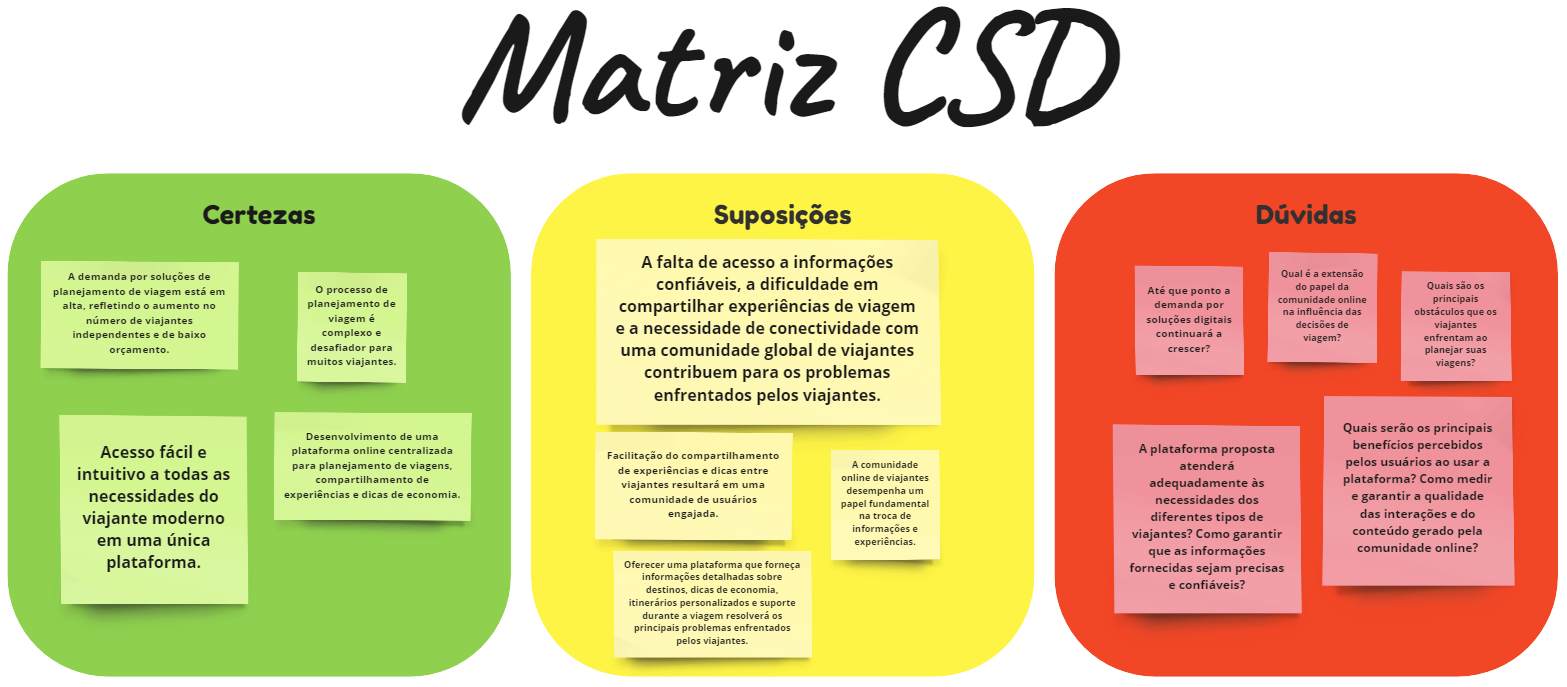
\includegraphics [width=1\textwidth]{IMGDOC/Matriz CSD.png}
      \label{csd imagem}
\end{figure}

{\subsection{Pesquisa com Google Forms / Pesquisa Quantitativa}}
Baseado na Matriz CSD, fizemos as seguintes perguntas para a pesquisa com o Forms:
\bigskip

O quanto você gosta de viajar?
\begin{figure}[H]
      \centering
      \includegraphics [width=1\textwidth]{IMGDOC/Quanto Gosta.png}
      \label{Pesquisa1}
\end{figure}

Quando você viaja, você posta nas redes sociais?
\begin{figure}[H]
      \centering
      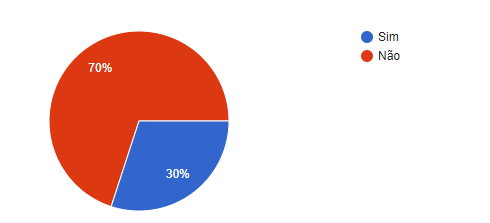
\includegraphics [width=1\textwidth]{IMGDOC/Redes sociais.png}
      \label{Pesquisa2}
\end{figure}

Você já teve dificuldades para planejar uma viagem?
\begin{figure}[H]
      \centering
      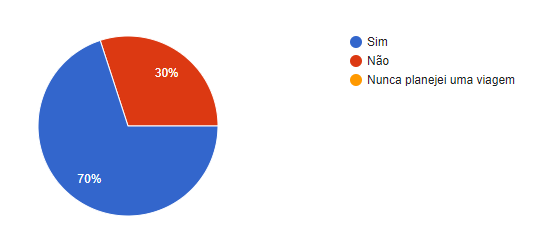
\includegraphics [width=1\textwidth]{IMGDOC/Dificuldades planejar.png}
      \label{Pesquisa3}
\end{figure}

Quando planejou a viagem, você demorou muito para planejar?
\begin{figure}[H]
      \centering
      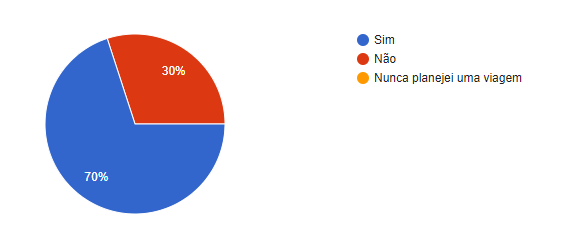
\includegraphics [width=1\textwidth]{IMGDOC/Demora planejar.png}
      \label{Pesquisa4}
\end{figure}

Você já teve muitas dificuldades para achar lugares baratos e confiáveis quando estava viajando?
\begin{figure}[H]
      \centering
      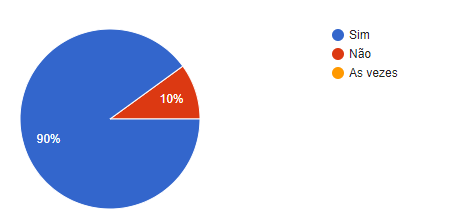
\includegraphics [width=1\textwidth]{IMGDOC/Dificuldades achar.png}
      \label{Pesquisa5}
\end{figure}

Baseado nas perguntas que você respondeu, você gostaria e acharia útil um site ou um app para uma comunidade de viajantes, feito para todos se ajudarem?
\begin{figure}[H]
      \centering
      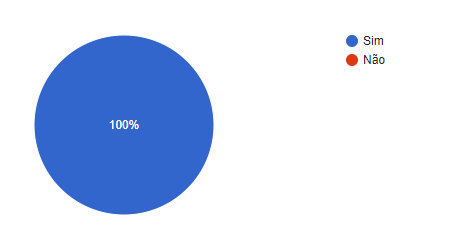
\includegraphics [width=1\textwidth]{IMGDOC/Fim pesquisa.png}
      \label{Pesquisa6}
\end{figure}

Algumas pessoas que participaram:
\begin{figure}[H]
      \centering
      \includegraphics [width=0.5\textwidth]{IMGDOC/participantes.png}
      \label{Pesquisa7}
\end{figure}


{\subsection{Entrevista / Pesquisa Qualitativa}}
Pesquisa feita no dia 15/04, às 15:36. Nome do participante: Kayk Cesar

Resumo:

"- Você gosta muito de viajar?"

"- Gosto bastante. Para mim, é uma das melhores experiências que podemos ter, explorar novos lugares e culturas."

"- Você já passou por algum desafio quando foi planejar alguma viagem?"

"- Sim, já tive algumas dificuldades ao planejar viagens. Às vezes, é complicado conciliar horários, encontrar acomodações adequadas e decidir quais atividades incluir no itinerário.
Já passei por algumas experiências em que eu não conseguia achar lugares baratos. Especialmente em destinos desconhecidos, pode ser difícil discernir entre opções que oferecem um bom custo-benefício e aqueles que são apenas uma armadilha para turistas."

"- Você acha que deveria ter algo para ajudar pessoas a não passar por essas dificuldades?"

" -Com base nas minhas experiências, acho que um site ou aplicativo para a comunidade de viajantes seria extremamente útil. Seria ótimo ter um espaço onde as pessoas possam compartilhar dicas, recomendações, experiências e até mesmo oferecer ajuda mútua durante o processo de planejamento de viagens."


\begin{enumerate}
      \item Qual o objetivo da Matriz CSD e das pesquisas quantitativa e qualitativa?

            A Matriz CSD é uma estrutura para avaliar e comparar opções, considerando critérios importantes, possíveis substitutos e decisões a serem tomadas. Já as pesquisas quantitativa e qualitativa têm objetivos um pouco distintos: a quantitativa coleta dados numéricos para análise estatística, enquanto a qualitativa busca compreender profundamente os significados subjacentes aos dados. Ambas fornecem insights essenciais para embasar decisões, seja por meio de análises numéricas ou compreensão aprofundada do contexto e das necessidades dos usuários.

      \item Qual a estratégia adotada pelo time Wanderlust para fazer a Matriz CSD?

            Nosso time adotou uma abordagem colaborativa e estruturada para criar a Matriz CSD. Começamos identificando criteriosamente os critérios essenciais para avaliar as opções em análise. Em seguida, discutimos potenciais substitutos para cada opção e refletimos sobre as decisões cruciais a serem tomadas. Ponderamos a importância de cada critério e os classificamos por relevância. Durante reuniões de equipe, revisamos os resultados, buscando chegar a um consenso sobre as melhores opções. Opcionalmente, buscamos feedback externo para validar nossas conclusões. Essa abordagem nos permitiu desenvolver uma Matriz CSD abrangente e bem fundamentada, fornecendo uma estrutura sólida para tomada de decisões informadas.

      \item Qual a estratégia adotada pelo time Wanderlust para fazer as pesquisas?

            Nosso time adotou uma abordagem abrangente para conduzir pesquisas quantitativa e qualitativa. Começamos definindo claramente os objetivos da pesquisa e planejando a amostra para garantir sua representatividade. Para a quantitativa usamos o Google Forms, com um questionário estruturado para a pesquisa e espalhamos em grupos de telegram. Para a qualitativa criamos um roteiro de entrevista e escolhemos uma pessoa para fazê-la. Interpretamos os resultados para gerar insights significativos e preparamos relatórios detalhados para compartilhar com a equipe e outras partes interessadas.

      \item Qual o resultado alcançado?

            Essa abordagem nos permitiu obter insights valiosos para informar nossas decisões e estratégias. Também foi usada para definir se o nosso projeto pode satisfazer e tirar dores dos nossos usuários.

      \item Qual a análise do time Wanderlust pela visão do design?

            Com os resultados obtidos, a análise que tivemos foi que, o design vai ter que fazer a página de publicações bem definida e com um sistema de avaliação para os usuários sempre terem o melhor resultado.

\end{enumerate}
\bigskip

\section{Benchmark}
De acordo com pesquisas feitas em sites e redes sociais, os concorrentes tem dificuldades em alguns aspectos, trivago e mochileiros.com não postam muito em suas redes sociais.
Trivago tem problemas com o desempenho de seus sites, já mochileiros.com tem problemas com o desempenho e com sua acessibilidade em seu site.

\subsection{Gráficos Trivago}

\begin{figure}[H]
      \centering
      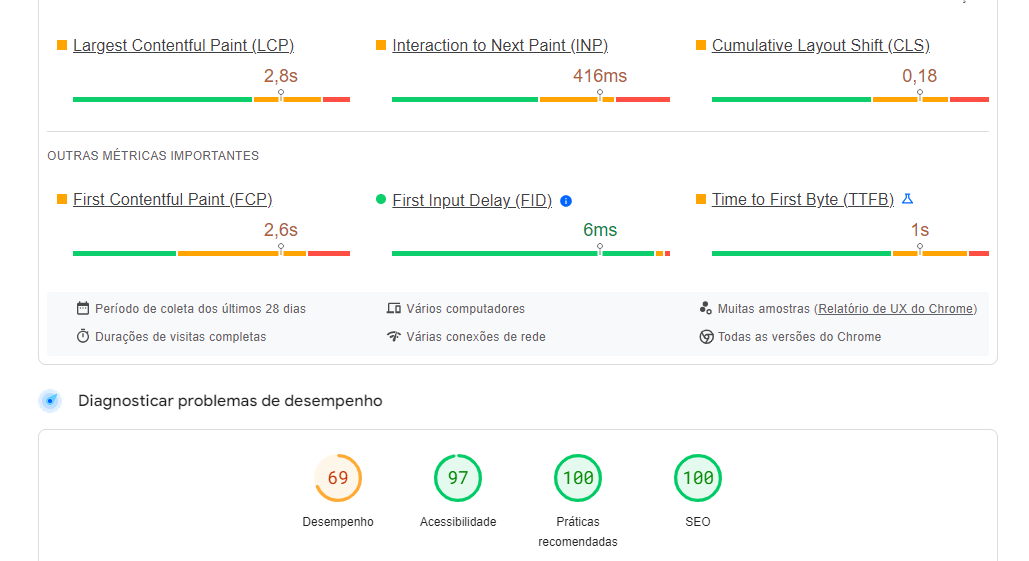
\includegraphics [width=1\textwidth]{IMGDOC/AnaliseTrivago1.png}
      \label{pesq1 tri}
\end{figure}
\begin{figure}[H]
      \centering
      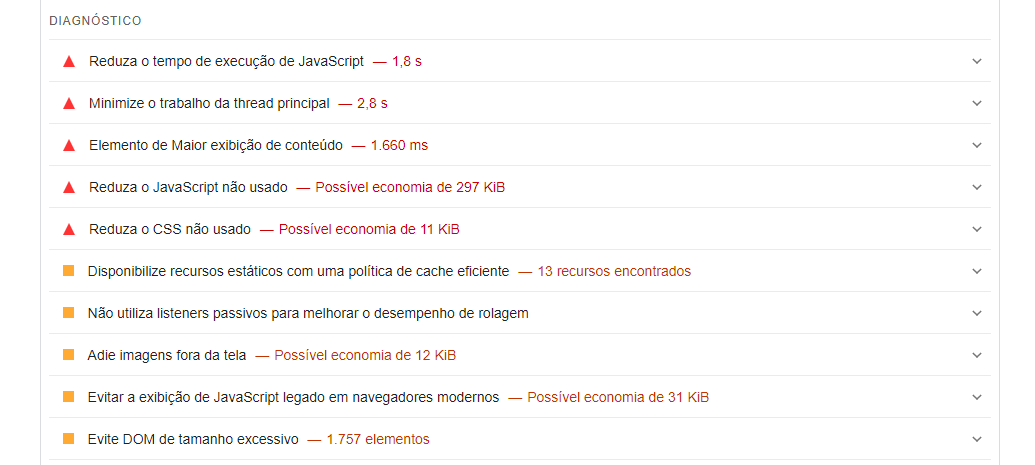
\includegraphics [width=1\textwidth]{IMGDOC/AnaliseTrivago2.png}
      \label{pesq2 tri}
\end{figure}

\subsection{Gráficos Mochileiros.com}

\begin{figure}[H]
      \centering
      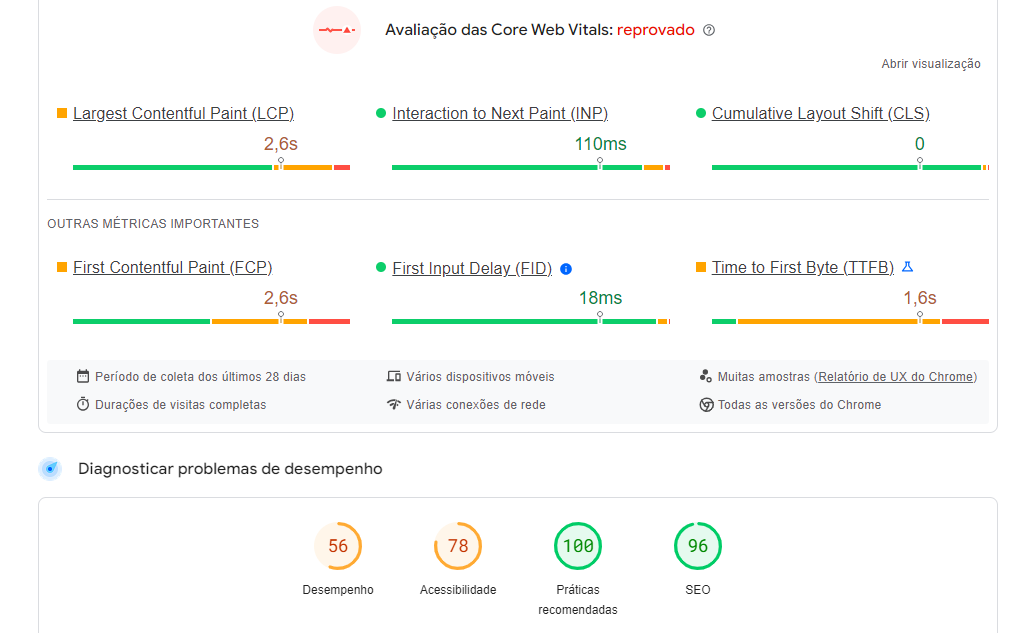
\includegraphics [width=1\textwidth]{IMGDOC/AnaliseMochileiros1.png}
      \label{pesq1 mochi}
\end{figure}
\begin{figure}[H]
      \centering
      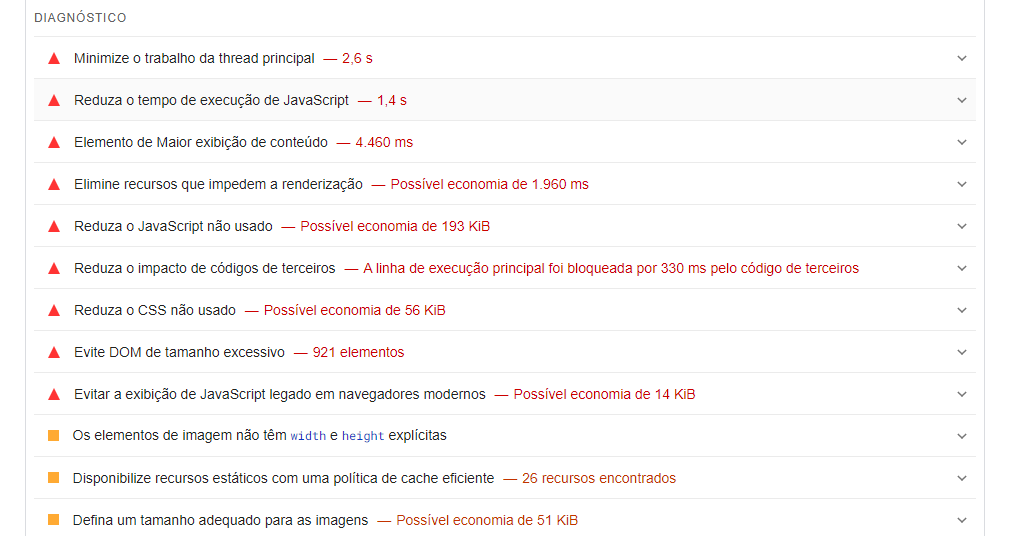
\includegraphics [width=1\textwidth]{IMGDOC/AnaliseMochileiros2.png}
      \label{pesq2 mochi}
\end{figure}

\begin{enumerate}
      \item Qual o objetivo do Benchmark?

            O objetivo do Benchmark é comparar o desempenho, práticas e resultados de uma organização, produto ou serviço com os de outros similares no mercado. Isso permite identificar áreas de excelência, oportunidades de melhoria e lacunas em relação à concorrência. O benchmarking pode ser utilizado para impulsionar a inovação, aprimorar processos, aumentar a eficiência e a competitividade, além de fornecer insights valiosos para orientar decisões estratégicas. Em resumo, o benchmarking visa alcançar a excelência por meio da comparação e adaptação das melhores práticas e resultados observados no mercado.

      \item Qual a estratégia adotada pelo time Wanderlust para fazer o Benchmark?

            Nosso time realizou o benchmarking com sucesso, adotando uma abordagem estruturada e colaborativa. Começamos definindo claramente nossos objetivos e o escopo da análise. Em seguida, identificamos referências relevantes em nosso mercado ou indústria, buscando organizações e serviços que são reconhecidos como líderes ou exemplos de excelência ou que se pareçam com o que queremos fazer de projeto. Durante a coleta de dados, utilizamos, relatórios públicos e análises de mercado, garantindo que tivéssemos uma visão abrangente das práticas e desempenho das referências selecionadas. Ao analisar e comparar os dados, procuramos identificar padrões, tendências e diferenças significativas entre nossos próprios resultados e os das referências. Isso nos permitiu identificar insights valiosos e melhores práticas que poderíamos aplicar em nosso próprio projeto. Com base nessas descobertas, desenvolvemos planos de ação claros e viáveis para implementar melhorias em áreas específicas. Além disso, estabelecemos um processo de monitoramento contínuo para avaliar o progresso e ajustar nossas estratégias conforme necessário.

      \item Qual o resultado alcançado?

            Essa abordagem nos permitiu aprender com os líderes do mercado e sites parecidos para impulsionar a excelência em nosso próprio projeto.

      \item Qual a análise do time Wanderlust pela visão do design?

            Com os resultados obtidos o design terá que ser um design que possa ter um desempenho e acessibilidade melhor ou similar aos dos outros sites.

\end{enumerate}


\section{Mapa da jornada do usuário}
\subsection{Sem a aplicação}

\begin{figure}[H]
      \centering
      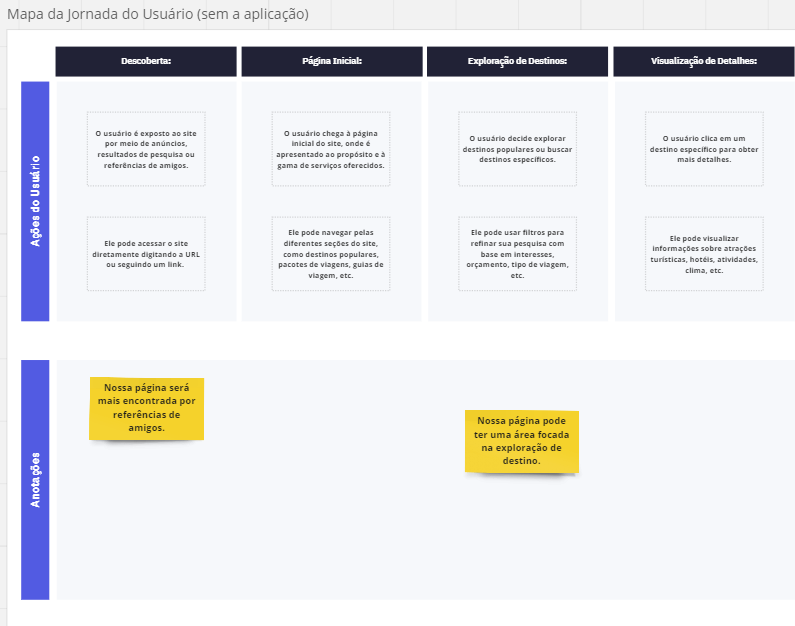
\includegraphics [width=1\textwidth]{IMGDOC/MapaSemA1.png}
      \label{mapa sem a1}
\end{figure}
\begin{figure}[H]
      \centering
      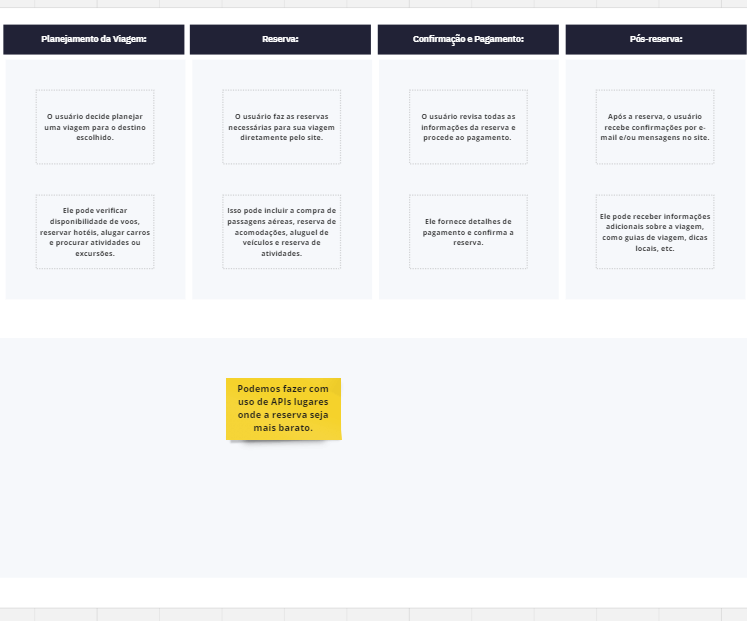
\includegraphics [width=1\textwidth]{IMGDOC/MapaSemA2.png}
      \label{mapa sem a2}
\end{figure}\begin{figure}[H]
      \centering
      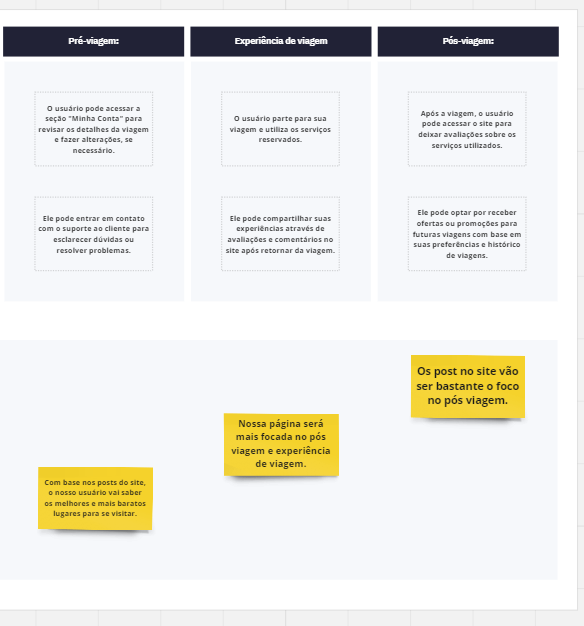
\includegraphics [width=1\textwidth]{IMGDOC/MapaSemA3.png}
      \label{mapa sem a3}
\end{figure}

\subsection{Com a aplicação}


\begin{enumerate}
      \item Qual o objetivo do Mapa da Jornada do Usuário?



      \item Qual a estratégia adotada pelo time Wanderlust para fazer o mapa?



      \item Qual o resultado alcançado?



      \item Qual a análise do time Wanderlust pela visão do design?



\end{enumerate}

\section{Rabiscoframes}



\begin{enumerate}
      \item Qual o objetivo dos Rabiscoframes?

            O objetivo dos rabiscoframes, ou wireframes de baixa fidelidade, é criar representações visuais simples e rápidas das interfaces de usuário, geralmente utilizando esboços ou desenhos básicos. Eles servem para explorar rapidamente conceitos, estruturas e fluxos de navegação de um projeto, sem se preocupar com detalhes visuais ou de design. Os rabiscoframes são úteis para comunicar ideias, obter feedback inicial e iterar rapidamente no processo de design, antes de investir tempo e recursos na criação de protótipos mais detalhados.

      \item Qual a estratégia adotada pelo time Wanderlust para fazer o Rabiscoframe?

            Nosso time criou rabiscoframes de forma eficaz, adotando uma abordagem estruturada. Começamos com sessões de brainstorming para gerar ideias e definimos objetivos claros para o projeto. Utilizamos esboços rápidos à mão, iterando e refinando-os com base no feedback da equipe. Documentamos os esboços de forma sucinta e os compartilhamos com as partes interessadas, garantindo uma compreensão comum do conceito. Revisamos os rabiscoframes antes de avançar para as próximas etapas do projeto.

      \item Qual o resultado alcançado?

            Essa abordagem nos permitiu explorar e comunicar ideias rapidamente, facilitando o desenvolvimento subsequente do projeto.

      \item Qual a análise do time Wanderlust pela visão do design?

            O design vai usar o rabiscoframe para ter de base para fazer o wireframe, porém ele não vai se basear totalmente nisso e algumas coisas vão ser adaptadas.

\end{enumerate}

\section{Wireframes e StyleGuide}
Link do Figma: https://www.figma.com/design/moQhturIxW4SQgz3IZib6S/Wireframe-e-Styleguide?t=GJ7Wh7Qk90H3Gi74-1

\begin{enumerate}
      \item Qual o objetivo do Wireframe e do StyleGuide?

            O objetivo do wireframe é criar um esboço visual básico de uma interface de usuário, representando a estrutura e o layout de uma página ou aplicativo antes do design final. Ele ajuda a visualizar a distribuição de elementos, o fluxo de navegação e a hierarquia de informações, permitindo que os designers e desenvolvedores experimentem diferentes ideias e refinem a interface de forma iterativa.
            O objetivo do Style Guide (Guia de Estilo) é estabelecer diretrizes de design consistentes para um projeto, definindo elementos visuais como cores, tipografia, ícones, espaçamento e outros aspectos de design. Ele fornece uma referência centralizada para garantir a coesão visual em todas as partes do projeto e entre diferentes membros da equipe. O Style Guide ajuda a manter a consistência visual, economizando tempo e esforço durante o processo de design e desenvolvimento, além de fortalecer a identidade da marca.

      \item Qual a estratégia adotada pelo time Wanderlust para fazer o Wireframe?

            Nosso time adotou uma abordagem cuidadosa e iterativa para criar wireframes. Começamos definindo claramente nossos objetivos e requisitos, garantindo uma compreensão sólida do que precisávamos alcançar. Em seguida, exploramos diferentes ideias e layouts através de esboços iniciais, permitindo-nos experimentar livremente antes de nos comprometermos com um design específico. Conforme refinávamos nossas ideias, passamos para ferramentas digitais para criar versões mais detalhadas dos wireframes. Durante todo o processo, buscamos feedback da equipe e partes interessadas, ajustando os designs conforme necessário. Além disso, realizamos testes de usabilidade para garantir que os wireframes atendessem às necessidades dos usuários. Finalmente, documentamos cuidadosamente nossos wireframes e os compartilhamos com a equipe para garantir uma compreensão clara e alinhada do design.

      \item Qual a estratégia adotada pelo time Wanderlust para fazer o StyleGuide?

            Nosso time desenvolveu o Style Guide de forma abrangente e eficaz. Começamos definindo objetivos e escopo claros, seguido pela identificação e estabelecimento de diretrizes para os elementos visuais, como cores, tipografia e ícones. Criamos exemplos e referências visuais para ilustrar as diretrizes, garantindo sua compreensão e aplicabilidade. Organizamos todas as informações em um documento centralizado, facilitando o acesso e compreensão por parte da equipe. Após revisão e feedback, iteramos no Style Guide, garantindo sua clareza e precisão.

      \item Qual o resultado alcançado?

            A abordagem do Wireframe foi colaborativa e centrada no usuário nos permitiu criar wireframes eficazes que serviram como uma base sólida para o desenvolvimento posterior da interface do usuário. Já a abordagem do StyleGuide garantiu consistência visual e coesão em todas as partes do projeto.

      \item Qual a análise do time Wanderlust pela visão do design?

            Com os resultados obtidos, o design do nosso site deve ser feito com base no style guide e no wireframe. Sempre seguindo essas duas bases e utilizando a criatividade.

\end{enumerate}

\section{Protótipo de Alta fidelidade}
Link do Figma: https://www.figma.com/design/PQnKKkcY3oaeLRCQjt7QCQ/Protótipo-de-alta-resolução?t=BZq9l4zKQ17pxqpl-0

\begin{enumerate}
      \item Qual o objetivo o Protótipo de Alta fidelidade?

            O objetivo do protótipo de alta fidelidade é criar uma representação visual detalhada e interativa da interface de usuário final de um produto ou sistema. Ele visa simular fielmente a aparência, interação e funcionalidade da interface, proporcionando uma experiência próxima do produto final. Isso permite que os designers e desenvolvedores testem e refinem a usabilidade, identifiquem problemas de design e comuniquem efetivamente suas ideias para as partes interessadas. O protótipo de alta fidelidade é uma etapa crucial no processo de design, ajudando a validar conceitos, reduzir riscos e acelerar o desenvolvimento do projeto/produto.

      \item Qual a estratégia adotada pelo time Wanderlust para fazer o Protótipo?

            Nosso time adotou uma abordagem cuidadosa e estruturada para criar protótipos de alta fidelidade. Começamos definindo objetivos claros e o escopo da interface a ser prototipada. Em seguida, utilizamos o Figma para desenvolver o design visual e implementar componentes interativos. Pesquisamos e coletamos feedback, buscando oportunidades de melhoria, garantindo que o protótipo atendesse às expectativas e requisitos do usuário

      \item Qual o resultado alcançado?

            Essa abordagem nos permitiu criar um protótipo eficaz que representa fielmente a interface final do nosso site.

      \item Qual a análise do time Wanderlust pela visão do design?

            No nosso protótipo de alta fidelidade, foi feito da melhor maneira possível e semore seguindo tudo que foi passado, principalmente o style guide e os wireframes.

\end{enumerate}

\section{Avaliação Heurística}

\begin{enumerate}
      \item Qual o objetivo da Avaliação Heurística?



      \item Qual a estratégia adotada pelo time Wanderlust para fazer a avaliação?



      \item Qual o resultado alcançado?



      \item Qual a análise do time Wanderlust pela visão do design?



\end{enumerate}


\end{document}
